\documentclass{beamer}

\usepackage{beamerthemesplit}
\usetheme{Singapore}

\input{../../include/preamble.inc} 
\input{../../include/definitions.inc} 
\input{../../include/author.inc} 

\title[]{Течения газа в сужающейся трубке тока. Элементарная теория сопла Лаваля}

\begin{document}
	
\frame[plain]{\titlepage}

\frame[plain]{
	\frametitle{Аннотация}
	\parbox{\textwidth}{
		Трубка тока. Постоянство расхода газа в трубке тока для стационарных течений. Сжимаемость трубок тока. Простое сопло, сопло Лаваля. Истечение газа из простого сопла. 
		Элементарная теория сопла Лаваля. 
	}
}

\frame{
	\frametitle{Трубка тока}
	
	\begin{dfn}
		\parbox{\textwidth}{
			\alert{Трубкой тока} называется поверхность, образованная линиями тока,  построенными из некоторой замкнутой кривой. 
		}
	\end{dfn}

	
	\centering\bigskip
	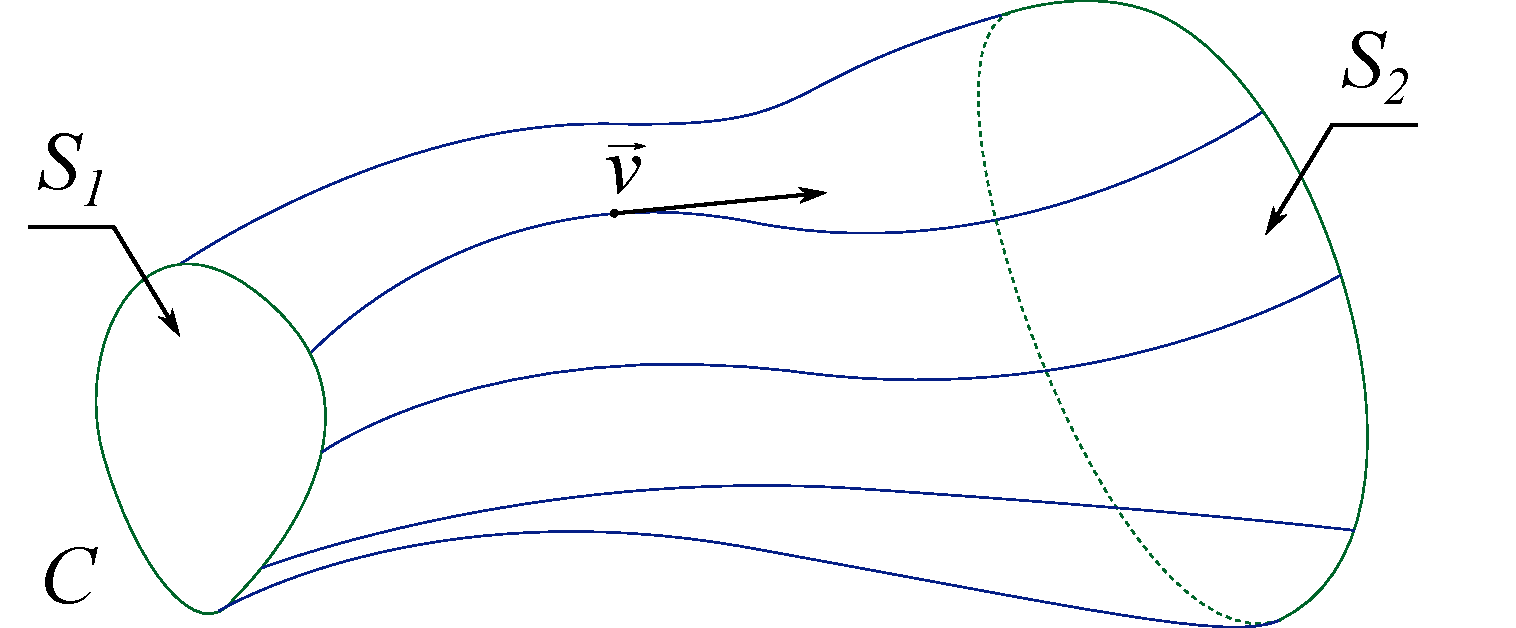
\includegraphics[width=0.7\linewidth]{../img/tube.pdf}
	
}


\frame{
	\frametitle{Постоянство расхода для трубки тока}


	\begin{exampleblock}{Закон сохранения массы в трубке тока}
		\parbox{\textwidth}{
			Закон сохранения массы имеет вид:
			\[
			\pd{\rho}{t} + \divo ( \rho \vec{v} )  = 0.
			\]
			Для стационарного течения:  $\divo (\rho \vec{v}) = 0$.
		}
	\end{exampleblock}
	\begin{theorems}
		\normalfont
		\parbox{\textwidth}{
			Для стационарного течения расход газа через любое поперечное сечение трубки тока имеет одну и ту же величину:
			\[
			 \int_{S_1} \rho v_n dS = \int_{S_2} \rho v_n dS,
			\]
			где $S_1$, $S_2$ -- различные сечения трубки тока. 
		}
	\end{theorems}
}


\frame{
	\frametitle{Постоянство расхода для трубки тока}
	\begin{proof}
		\parbox{\textwidth}{
			\begin{columns}

				\begin{column}{0.3\textwidth}
					\parbox{\textwidth}{
						Пусть далее 
						\[
						\vec{a} = \rho\vec{v},
						\]
						тогда
					}
				\end{column}
				\begin{column}{0.7\textwidth}
					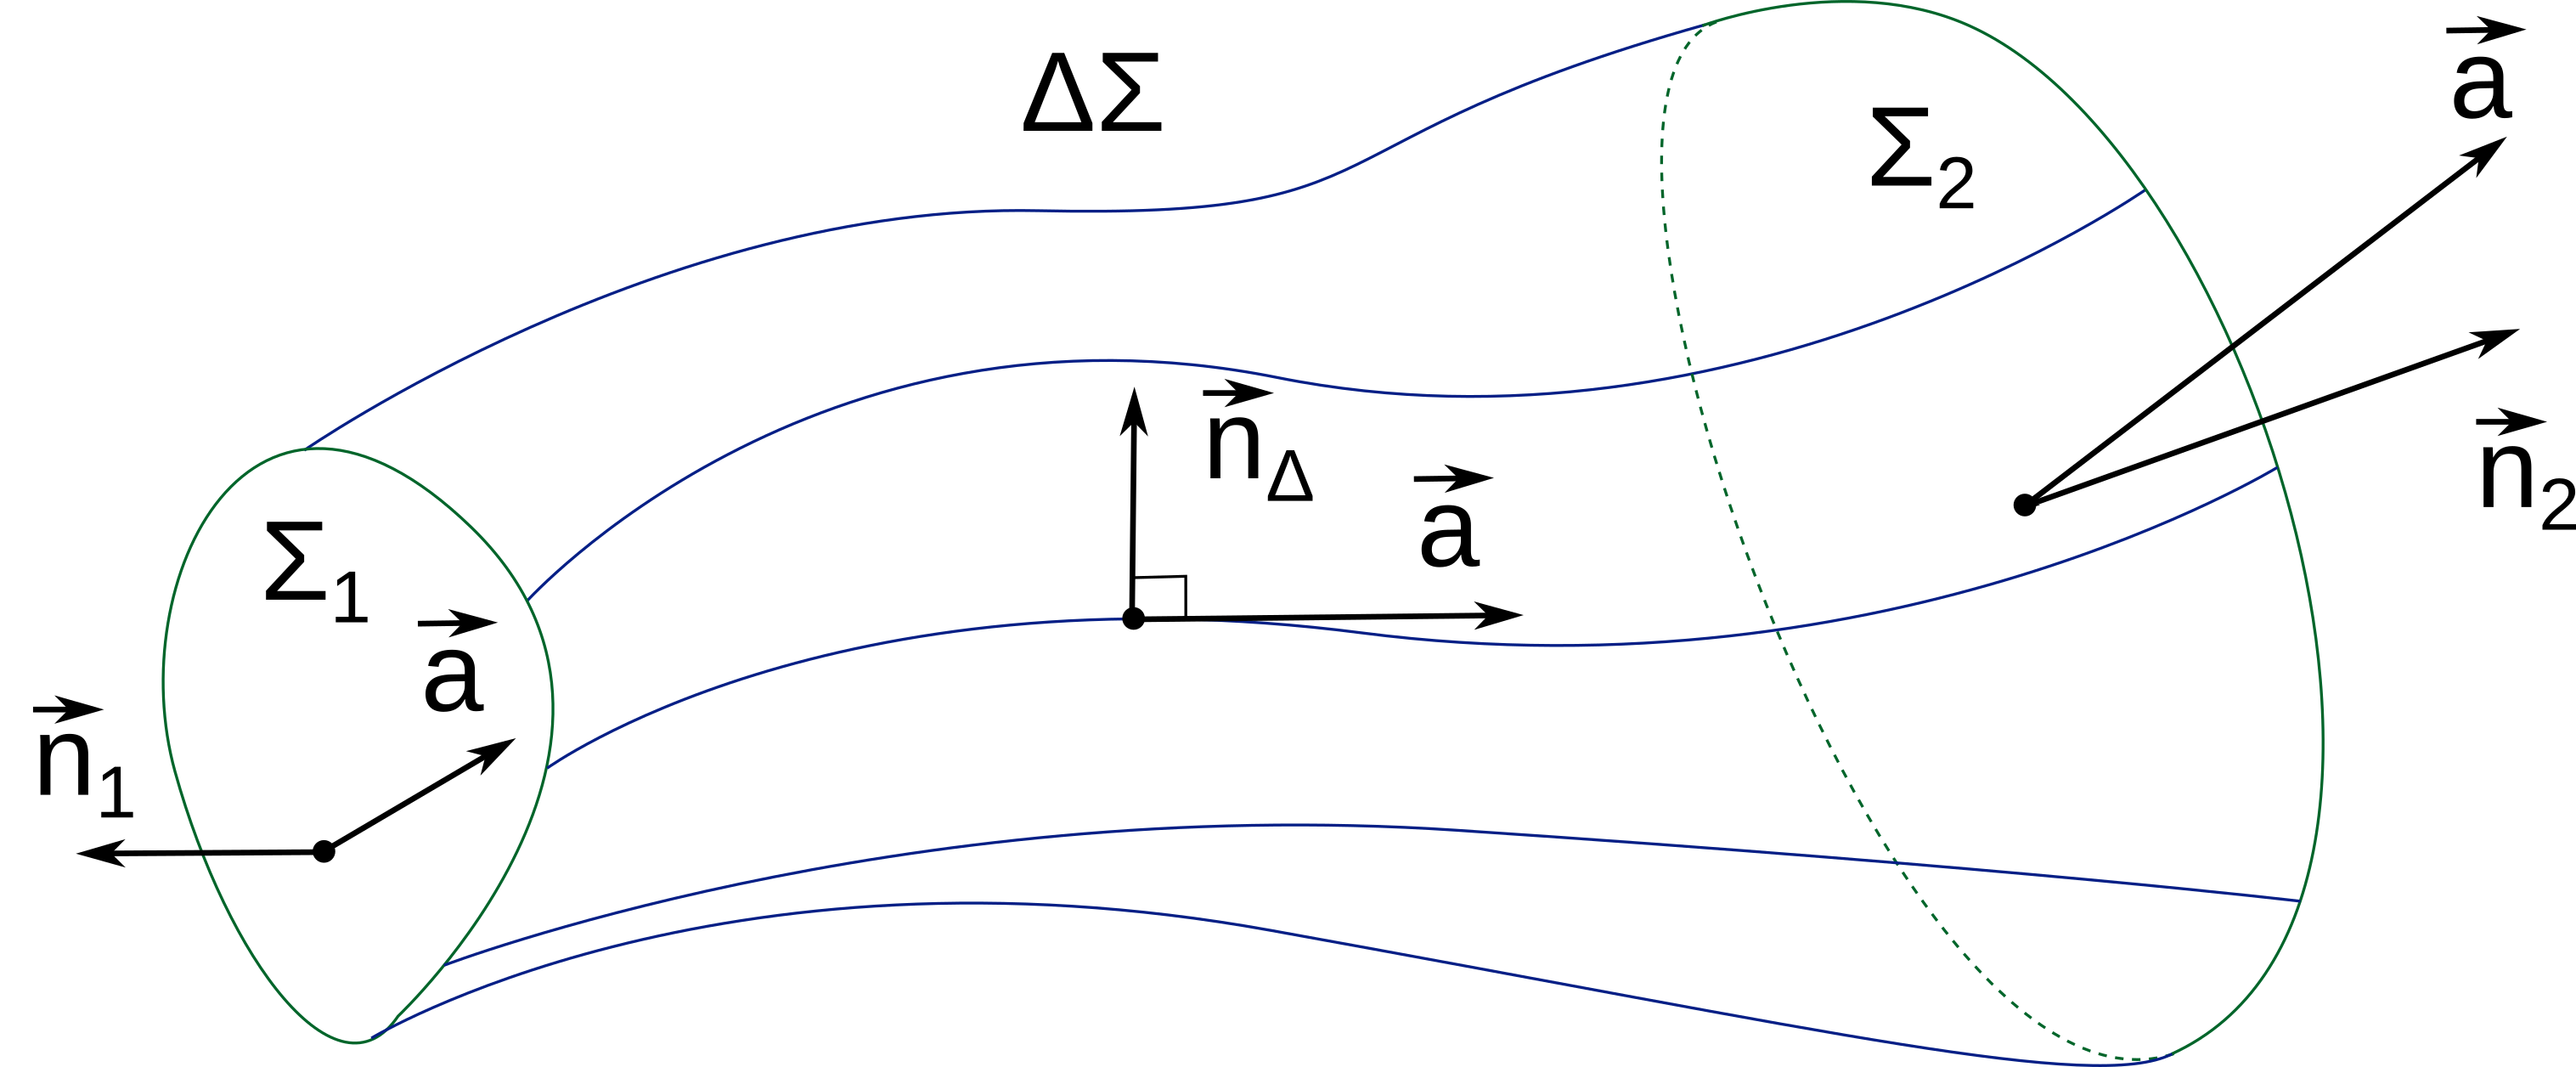
\includegraphics[width=\textwidth]{../img/solenoid.png}
				\end{column}			
			\end{columns}
			\[
			0=\int\limits_V\divo{\vec{a}}dV= \pause 
			\int\limits_{\Sigma}\vec{a}\cdot\vec{n}dS= \pause 
			\int\limits_{\Sigma_1}\vec{a}\cdot\vec{n}_1 dS+
			\int\limits_{\Delta\Sigma}\vec{a}\cdot\vec{n}_\Delta dS+
			\int\limits_{\Sigma_2}\vec{a}\cdot\vec{n}_2 dS.
			\] \pause 
			Отсюда  $\int\limits_{\Sigma_1}\vec{a}\cdot\vec{n}_1 dS=-\int\limits_{\Sigma_2}\vec{a}\cdot\vec{n}_2 dS$, \pause 
			т.к. $\int\limits_{\Delta\Sigma}\vec{a}\cdot\vec{n}_\Delta dS=0$ в силу ортогональности векторов $\vec{a}$ и $\vec{n}_\Delta$,  \pause т.е. потоки вектора $\vec{a}$ через $\Sigma_1$ и $\Sigma_2$ совпадают.
		}
	\end{proof}
}


\frame{
	\frametitle{Сжимаемость трубок тока}
	
	\centering
	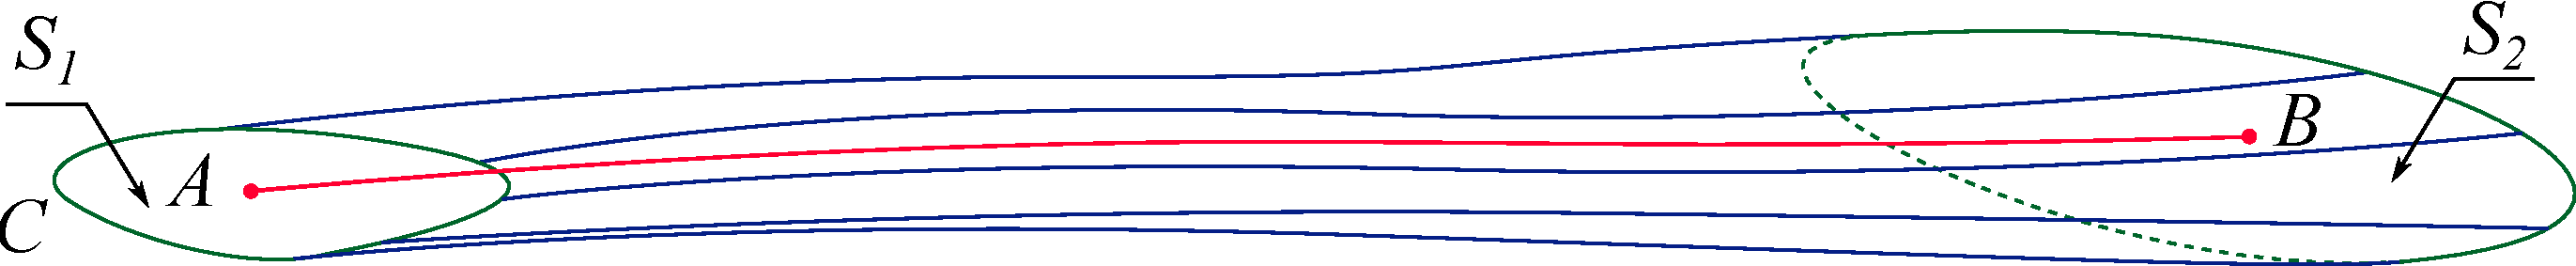
\includegraphics[width=0.9\linewidth]{../img/slim_tube.pdf}
	
	\bigskip
	
	\begin{exampleblock}{Основные предположения}
		\parbox{\textwidth}{
		Далее будем рассматривать очень узкие трубки тока, для которых можно считать, что параметры $\rho$, $p$, $c$ и $\vec{v}$ мало меняются по ее сечению, построенному перпендикулярно выделенной линии тока (на рисунке $AB$), а рассматриваемое течение изоэнтропическое.
		}	
	\end{exampleblock}\pause

	\begin{exampleblock}{Соотношения на выделенной линии тока}
		\parbox{\textwidth}{
			Параметризовав линию тока $AB$, можно записать закон сохранения массы и интеграл Бернулли для параметров течения:			
			\[
			\rho v S = C_1,\quad
			\frac{v^2}{2} + \frac{c^2}{\gamma-1} = C_2.
			\]
		}
	\end{exampleblock}


	
}

\frame{
	\frametitle{Сжимаемость трубок тока }
	
	\begin{exampleblock}{Соотношение для параметров течения в дифференциалах}
		\parbox{\textwidth}{
			\[
			\frac{d\rho}{\rho} + \frac{dv}{v} + \frac{dS}{S} = 0,\quad
			v\, dv + \frac{2 c}{\gamma-1}\, dc  = 0.
			\]
		}
	\end{exampleblock}\pause

	\begin{exampleblock}{Дополнительные соотношения}
		\parbox{\textwidth}{
			Так как для изоэнтропических течений $dp = c^2 \, d\rho$ и $c^2 = \displaystyle\frac{\gamma p}{\rho}$, то рассмотрим дифференциал от последнего:
			\[
				2c\, dc =
				\frac{\gamma}{\rho}\, dp - \frac{\gamma p}{\rho^2}\,d\rho = 
				(\gamma -1) c^2 \frac{d\rho}{\rho}.
			\]
			Подставляя дополнительные соотношения в интеграл Бернулли в дифференциалах, получим:
			\[
				v\, dv +c^2 \frac{ d\rho }{\rho} = 0.
			\]
			
		}
	\end{exampleblock}
}

\frame{
	\frametitle{Сжимаемость трубок тока}
	
	\begin{exampleblock}{Связь между скоростью, сечением и числом Маха}
	\parbox{\textwidth}{
	Исключая из последнего выражения $d\rho/\rho$ с помощью закона сохранения массы в дифференциалах, получим \alert{уравнение Гюгонио}:
	\[
	(M^2-1) \,\frac{dv}{v} = \frac{dS}{S} \quad (v > 0), 
	\]
	где $M=v/c$ -- число Маха.
	}

	\begin{columns}
		\begin{column}{0.33\textwidth}
		\[ 
		M < 1
		\]	
		\end{column}
		\begin{column}{0.33\textwidth}
		\[ 
		M  = 1
		\]
		\end{column}
		\begin{column}{0.33\textwidth}
		\[ 
		M > 1
		\]	
		\end{column}
	\end{columns}
		
	\begin{columns}
		\begin{column}{0.33\textwidth}

		$dv < 0 \iff dS > 0$\\
		$dv  = 0 \iff dS = 0$\\
		$dv > 0 \iff dS < 0$
		
		\end{column}
		\begin{column}{0.33\textwidth}

		\centering
		$dS = 0$
		\end{column}
		\begin{column}{0.33\textwidth}

		$dv < 0 \iff dS < 0$\\
		$dv  = 0 \iff dS = 0$\\
		$dv > 0 \iff dS > 0$
		
		\end{column}
	
	\end{columns}
	\end{exampleblock}

%	\begin{exampleblock}{Связь площади трубки тока и скорости потока}
	\medskip
		\parbox{\textwidth}{
			Таким образом,
			$
			S(v) = \displaystyle\frac{C_1}{
				\rho^* v \left(
				1 - \displaystyle\frac{v^2}{v_{max}^2}
				\right)^{1/(\gamma-1)}
			}
			$.
		}
%	\end{exampleblock}
	
}

\frame{
	\frametitle{Сужающаяся и расширяющаяся трубка тока}
	
	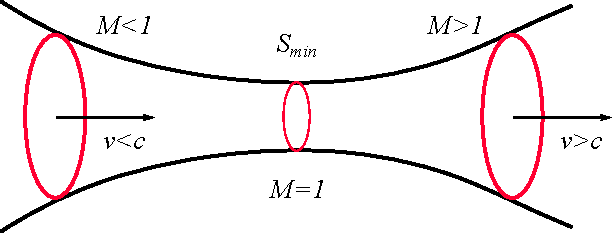
\includegraphics[width=\linewidth]{../img/tube_M.pdf}
	
}

\frame{
	\frametitle{ Простое сопло и сопло Лаваля }
	
	
	\begin{columns}
		\begin{column}{0.5\textwidth}
			\centering
			\small
			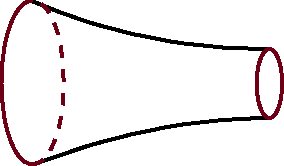
\includegraphics[width=0.5\linewidth]{../img/simple_nozzle.pdf}\\
			Простое сопло
		\end{column}
		\begin{column}{0.5\textwidth}
			\centering\small
			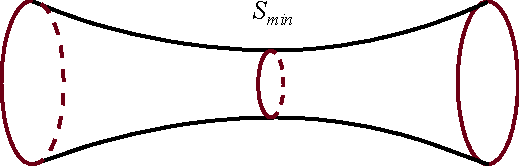
\includegraphics[width=\linewidth]{../img/Laval.pdf}\\
			Сопло Лаваля
		\end{column}
	\end{columns}

	\bigskip
	\begin{exampleblock}{}
		\parbox{\textwidth}{
			Насадок, предназначенный для адиабатического разгона потока от дозвуковых скоростей к сверхзвуковым, обладающий зоной сужения и расширения, называется \alert{соплом Лаваля}. Насадок, имеющий только зону сжатия, называется \alert{простым соплом}.
		}
	\end{exampleblock}

	
}


\frame{
	\frametitle{Связь между  параметрами газа в различных сечениях}
	
	\parbox{\textwidth}{
		

	
	\[
	\frac{S}{S_1} = \frac{\rho_1 v_1}{\rho v} = 
	\frac{M_1}{M}
	\left(
	\frac{
	1 + \displaystyle\frac{\gamma-1}{2} M^2
	}
	{
	1 +  \displaystyle\frac{\gamma-1}{2} M_1^2
	}
	\right)^{\frac{\gamma+1}{2(\gamma-1)}},
	\]
	\[
	\begin{array}{lcclcc}
	\displaystyle\frac{p}{p_1} & = & 
	\left(
	\displaystyle\frac{
		1 + \displaystyle\frac{\gamma-1}{2} M^2
	}
	{
		1 +  \displaystyle\frac{\gamma-1}{2} M_1^2
	}
	\right)^{\frac{\gamma}{\gamma-1}}, &
	\displaystyle\frac{\rho}{\rho_1} & = & 
	\left(
	\displaystyle\frac{
		1 + \displaystyle\frac{\gamma-1}{2} M^2
	}
	{
		1 +  \displaystyle\frac{\gamma-1}{2} M_1^2
	}
	\right)^{\frac{1}{\gamma-1}}, \\
	\displaystyle\frac{T}{T_1} & = &  
	\displaystyle\frac{
		1 + \displaystyle\frac{\gamma-1}{2} M^2
	}
	{
		1 +  \displaystyle\frac{\gamma-1}{2} M_1^2
	}, &
	\displaystyle\frac{v}{v_1} & = &
	\displaystyle\frac{M}{M_1}
	\left(
	\frac{
		1 + \displaystyle\frac{\gamma-1}{2} M^2
	}
	{
		1 +  \displaystyle\frac{\gamma-1}{2} M_1^2
	}
	\right)^{\frac{1}{2}}.
	\end{array}
	\]
		Эти формулы дают \alert{параметрическое решение} задачи о квазиодномерном изоэнтропическом стационарном газовом потоке в трубке тока (сопле) переменного сечения.
	}
}

\frame{
	\frametitle{Связь между  параметрами газа, в котором есть критическое сечение}
	
	\parbox{\textwidth}{
	Положим, что в сечении $S_1 = S_{min}$ реализуется $M_1 = 1$, тогда:
	
	\[
	\frac{S}{S_{min}}  = 
	\left(\frac{2}{\gamma+1}
	\right)^{\frac{\gamma+1}{2(\gamma-1)}}
	\frac{1}{M}
	\left(
		1 + \displaystyle\frac{\gamma-1}{2} M^2
	\right)^{\frac{\gamma+1}{2(\gamma-1)}} = \alert{\Theta^{-1}(M)},
	\]
	\[
	\begin{array}{lcc}
	\displaystyle\frac{p}{p_{\text{кр}}} & = & % p/p_кр
	\left[
	\displaystyle\frac{2}{\gamma+1}
	\left(
		1 + \displaystyle\frac{\gamma-1}{2} M^2
	\right)
	\right]^{-\frac{\gamma}{\gamma-1}}, \\
	\displaystyle\frac{\rho}{\rho_{\text{кр}}} & = &  % \rho/\rho_кр
	\left[
		\displaystyle\frac{2}{\gamma+1}
		\left(
			1 + \displaystyle\frac{\gamma-1}{2} M^2
		\right)
	\right]^{-\frac{1}{\gamma-1}}, \\
	\displaystyle\frac{T}{T_{\text{кр}}} & = &  % T / Tкр
	\left[
		\displaystyle\frac{2}{\gamma+1}
		\left(
			1 + \displaystyle\frac{\gamma-1}{2} M^2
		\right)
	\right]^{-1},\\
	\displaystyle\frac{v}{v_{\text{кр}}} & = &   % v / vкр
	M
	\left[
		\displaystyle\frac{2}{\gamma+1}
		\left(
			1 + \displaystyle\frac{\gamma-1}{2} M^2
		\right)
	\right]^{-\frac{1}{2}}.
	\end{array}
	\]
	
	}
	
}

\frame{
	\frametitle{Зависимость числа Маха от площади сечения для воздуха}
	
	\begin{columns}
		\begin{column}{0.6\textwidth}
			\centering
			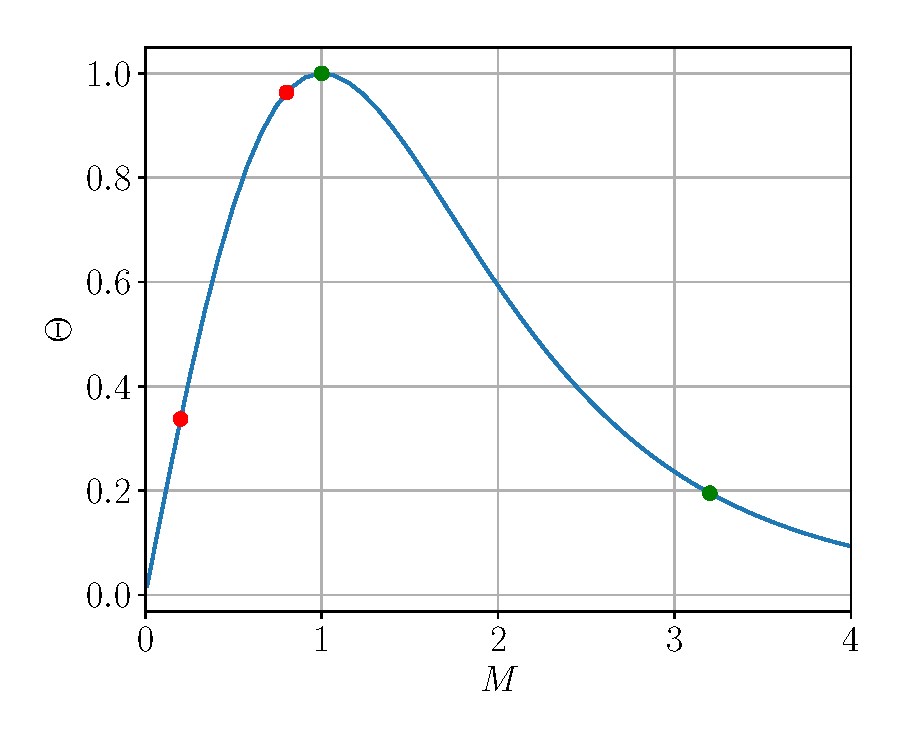
\includegraphics[width=\linewidth]{../img/M_theta.pdf}
			\[
			\frac{S_{min}}{S} = \Theta = \Theta(M)
			\]
		\end{column}
		\begin{column}{0.4\textwidth}
			\parbox{\textwidth}{
			
			Из рисунка следует, что для повышения числа $M$ от $0,2$ до $0,8$ газ должен пройти через конфузор с сечением, уменьшающимся в три раза. 
			
			\bigskip
			А чтобы увеличить $M$ от значения $1$ в критическом сечении до $3,2$, необходимо построить сверхзвуковой диффузор с площадью, в пять раз превышающую $S_{min}$.
			}
		\end{column}
	\end{columns}
}


\frame{
	\frametitle{Истечение газа через простое сопло}
	
	\begin{columns}
		\begin{column}{0.5\textwidth}
			\centering
			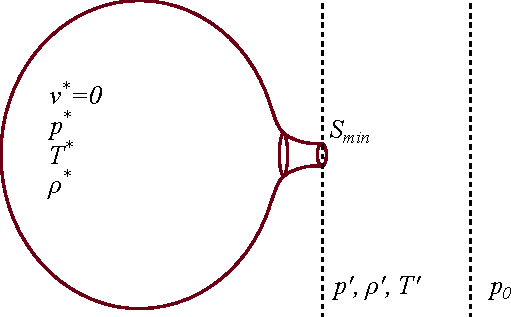
\includegraphics[width=\linewidth]{../img/simple_nozzle_flow.pdf}
		\end{column}
		\begin{column}{0.5\textwidth}
			\begin{exampleblock}{Постановка и решение задачи}
				\parbox{\textwidth}{
					
					\only<1>{					
					Рассмотрим истечение газа из емкости большого объема через конфузор с критическим сечением  $S_{min}$  и параметрами торможения газа вдали от сопла в емкости $p^*$, $\rho^*$, $T^*$. Противодавление снаружи равно $p_0$. Штрихами будем обозначать параметры на срезе сопла.
					}
				
					\only<2>{
					Пусть $m$ -- массовый расход газа через любое сечение сопла, тогда
					\[
					m = \rho v S = \rho' v' S_{min}.
					\]
					
 					Пусть $m_{\text{кр}} = \rho_{\text{кр}} v_{\text{кр}} S_{min}$ -- критическое значение массы, соответствующее числу Маха, равному $1$, тогда
 					\[
 						\frac{m}{m_{\text{кр}}} = \frac{\rho' v'}{\rho_{\text{кр}} v_{\text{кр}}} = \theta(M').
 					\]
				
					}
				
					\only<3>{
					Используя формулу
					\[
					p' = p^* \left(
						1 + \frac{\gamma-1}{2} M'^2
					\right)^{-\frac{\gamma}{\gamma-1}},
					\]	
					исключаем $M'$ из выражения для $m/m_{\text{кр}}$ и получаем:
				}
					
				}
			\end{exampleblock}

			
		\end{column}
	\end{columns}
	
	\only<3>{
	\bigskip
	\bigskip
	\[
	\frac{m}{m_{\text{кр}}} = \sqrt{
	\frac{2}{\gamma-1}
	\left(
		\frac{\gamma+1}{2}
	\right)^\frac{\gamma+1}{\gamma-1}
	\left(
		\frac{p'}{p^*}
	\right)^\frac{2}{\gamma}
	\left[
		1 - 
		\left(
			\frac{p'}{p^*}
		\right)^\frac{\gamma-1}{\gamma}	
	\right]
	}.
	\]	
	}

	
}



\frame{
	\frametitle{Истечение газа через простое сопло}
	
	\begin{columns}
		\begin{column}{0.5\textwidth}
			\centering
			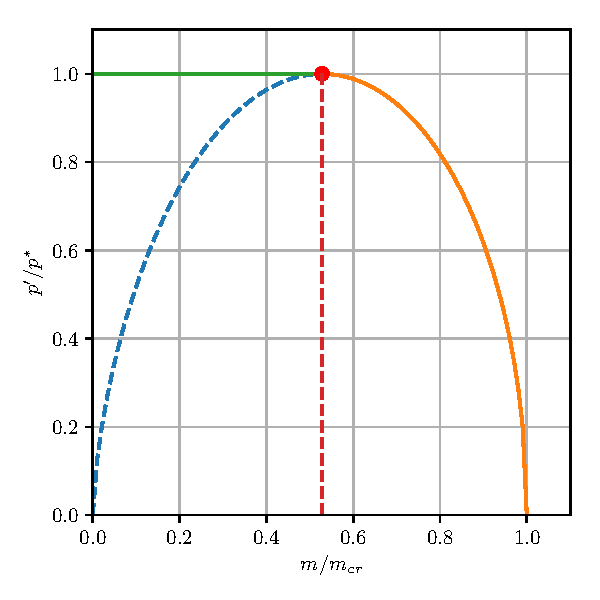
\includegraphics[width=\linewidth]{../img/simple_nozzle_m.pdf}
		\end{column}
		\begin{column}{0.5\textwidth}
			\begin{exampleblock}{Описание}
				\parbox{\textwidth}{
					\only<1>{
						При уменьшении $p_0$ до тех пор, пока течение на срезе сопла не станет звуковым, будет реализовываться режим, описываемый на графике оранжевой ветвью, и давление на выходе из сопла можно принимать равным противодавлению: 
						\[
						p'=p_0.
						\]
					}
				
					\only<2>{
						Как только  на срезе сопла  установится звуковое течение
						\[
						M'=1,
						\]
						то произойдет его запирание. В критическом сечении установятся критические параметры, которым соответствует максимальный возможный расход газа $m_{\text{кр}}$ (зеленая ветвь графика).				
					}
					
%					Как только давление на выходе станет критическим, то в минимальном сечении установится звуковое течение $M'=1$ 
				
					
				}
			\end{exampleblock}
			
			
		\end{column}
	\end{columns}
	
	\only<1>{
	\bigskip
	\[
	\frac{m}{m_{\text{кр}}} = \sqrt{
	\frac{2}{\gamma-1}
	\left(
	\frac{\gamma+1}{2}
	\right)^\frac{\gamma+1}{\gamma-1}
	\left(
	\frac{p'}{p^*}
	\right)^\frac{2}{\gamma}
	\left[
	1 - 
	\left(
	\frac{p'}{p^*}
	\right)^\frac{\gamma-1}{\gamma}	
	\right]
	}
	\]
	}

	\only<2>{
	\bigskip	
	\[
	x_{\text{кр}}=\frac{p_{\text{кр}}}{p^*} = \left( \frac{2}{\gamma+1} \right)^{\frac{\gamma}{\gamma-1}},\quad	
	m_{\text{кр}}	= 
%	\rho_{\text{кр}} v_{\text{кр}} S_{min} = 
	\left(
		\frac{2}{\gamma-1}
	\right)^\frac{\gamma+1}{2(\gamma-1)} 
	\sqrt{\gamma p^*\rho^*} S_{min}.
	\]
	}

	
}




%
%\frame{
%	\frametitle{Сжимаемость трубок тока}
%	\begin{exampleblock}{Связь между расходом и скоростью}
%	\parbox{\textwidth}{
%		Исключая из закона сохранения массы в дифференциалах $dS/S$ с помощью соотношения между скоростью, сечением и числом Маха, получим
%		\[
%		d(\rho v) = (1 - M^2) \rho \, dv. 
%		\]
%	}
%	
%	\begin{columns}
%		\begin{column}{0.35\textwidth}
%			\[ 
%			M < 1
%			\]	
%		\end{column}
%		\begin{column}{0.3\textwidth}
%			\[ 
%			M  = 1
%			\]
%		\end{column}
%		\begin{column}{0.35\textwidth}
%			\[ 
%			M > 1
%			\]	
%		\end{column}
%	\end{columns}
%	
%	\begin{columns}
%		\begin{column}{0.35\textwidth}
%			
%			$dv < 0 \iff d(\rho v) > 0$\\
%			$dv  = 0 \iff d(\rho v) = 0$\\
%			$dv > 0 \iff d(\rho v) < 0$
%			
%		\end{column}
%		\begin{column}{0.3\textwidth}
%			
%			\centering
%			$d(\rho v) = 0$
%		\end{column}
%		\begin{column}{0.35\textwidth}
%			
%			$dv < 0 \iff d(\rho v) < 0$\\
%			$dv  = 0 \iff d(\rho v) = 0$\\
%			$dv > 0 \iff d(\rho v) > 0$
%			
%		\end{column}
%		
%	\end{columns}
%	\end{exampleblock}
%	
%}


\frame{
	\frametitle{ Литература }
	\begin{literature} %[partopsep=1pt,label=\textbullet]
		\item 
		{\em Лойцянский~Л.\,Г.} 
		Механика жидкости газа и плазмы. Учеб. для вузов. --- 7-е изд., испр. -- М.: Дрофа, 2003.

		\item 
		{\em Седов~Л.\,И.} 
		Механика сплошной среды. Том 2. М.: Наука, 1970.
		
	\end{literature}
}

\end{document}
